\documentclass[12pt,a4paper]{article}
% Essential packages
\usepackage[utf8]{inputenc} % Character encoding
\usepackage{graphicx} % For images
\usepackage{amsmath} % For mathematical formulas
\usepackage{hyperref} % For hyperlinks
\usepackage{enumitem}
\usepackage{float} % For controlling figure placement

% Listings for code
\usepackage{xcolor} % For colored text
\usepackage{listings}

\definecolor{codegray}{rgb}{0.5,0.5,0.5}    % Colours for code
\definecolor{codegreen}{rgb}{0.0,0.6,0.0}
\definecolor{codeblue}{rgb}{0.13,0.13,1}
\definecolor{codepurple}{rgb}{0.58,0,0.82}
\definecolor{backcolor}{rgb}{0.95,0.95,0.92}

\lstset{    % Make listings look like code
  language=C,
  basicstyle=\ttfamily\small,
  backgroundcolor=\color{backcolor},
  commentstyle=\color{codegreen}\ttfamily,
  keywordstyle=\color{codeblue}\ttfamily\bfseries,
  stringstyle=\color{codepurple}\ttfamily,
  numberstyle=\tiny\color{codegray},
  numbers=left,
  numbersep=5pt,
  frame=single,
  breaklines=true,
  captionpos=b,
  showstringspaces=false,
  tabsize=2,
  morekeywords={cellauto}, % add extra keywords if needed
  morekeywords={apply_rule, reset, randomize, nachbar_check, random_auto},
  morekeywords={[2]<"structs.h">}, keywordstyle={[2]\color{codepurple}\ttfamily}
}

% Tighten space before sections
\usepackage{titlesec}
\titlespacing*{\section}{0pt}{0.5em}{0.5em}
\titlespacing*{\subsection}{0pt}{0.3em}{0.3em}
\setlength{\parindent}{0pt}

% Document metadata
\title{\textbf{Documentation Cellular Automats (Assignment 15)}}
\author{Mario Neuner, Christoph Bichlmeier, Jakob Guentner\\Leander Decristoforo}
\date{\today}
\begin{document}
\maketitle

\newpage
\tableofcontents
\pagebreak


% Problem A
\section{Part A: One Dimensional Cellular Automats}
\vspace{1cm}


\subsection{Task}
The task involves implementing a one-dimensional cellular automaton system that 
evolves through discrete time steps based on predefined rules. The automaton consists 
of a linear array of cells, each in state 0 or 1, where the next state is determined by 
a cell's current state and its immediate neighbors. The system must support four specific 
rules (22, 106, 187, 214) and handle two initialization modes: a determined start with a 1 
in the middle and zeros around and a random configuration. The program takes two command-line 
arguments, N for grid size and M for the number of time iterations and outputs the automaton's 
state after each iteration. These results can then be visualized using a separate plotting tool.
\newline

\vspace{1cm}


\subsection{Idea}
This project is built around a modular and rule-driven approach to simulating cellular automata. 
At the heart of the system is a structure called “cellauto”, which holds the key components of the 
simulation. It holds the current state of the grid, stored as a character array, the rule being applied 
encoded as an 8-bit pattern and parameters like the grid size N and number of iterations M.
\newline
The rules themselves are defined using arrays of eight characters, where each position corresponds to 
one of the possible neighborhood cell configurations (e.g., the pattern “111” maps to index “0”). During 
the simulation, the system updates the grid in steps. For each cell, considering its left, center, and right 
neighbors, wrapping around at the edges, determining the corresponding rule index, and updating the cell’s 
state based on the rule.
\newline
There are two modes of initialization implemented, one is determined, starting with a 
single 1 in the center and zeros around, and one random. 
The results of each simulation are saved in a format designed for easy visualization. 
Each line in the output file represents the complete state of the cells at a given time step.
\newline

\vspace{1cm}


\subsection{Implementation}
\subsection*{\small Data Structures and Rule Encoding}
At the core of the system is the \texttt{cellauto}-struct, defined in \texttt{structs.h}. This struct houses all the 
parameters and data needed to run a simulation, including the current state of the grid, the active rule, 
the simulation data, and the mode of initialization:
\newline
The rule definitions themselves are declared as global constants in \texttt{structs.h} and initialized in \texttt{structs.c}. 
Each rule is represented as an array of eight characters \texttt{(e.g., RULE\_22)}, corresponding to the eight possible 
arrangement of three cells. These arrays are indexed from 0 to 7, where each index corresponds to a specific 
neighborhood pattern. For instance, \texttt{Rule\_22 = \{0,0,0,1,0,1,1,0\}} defines the rule's response to configurations 
ranging from 111 with index 0 to 000 with index 7. 
\newline

\subsection*{\small State Management and Rule Application}
The evolution of the automaton is made by functions implemented in \texttt{cell.c}. Where two initialization modes are used. 
One Deterministic via \texttt{reset(cellauto *c)}, which sets a single active cell (1) at the center of the grid, and the other 
one Random via \texttt{randomize(cellauto *c)}, which assigns each cell a 0 or 1 at random, using \texttt{srand(time(NULL))}.
\newline
The key function that does the state transitions is \texttt{apply\_rule(cellauto *c)}. For each cell in the 
current state array, the function checks the left, center, and right neighbors using a series of \texttt{if} statements. 
Each possible pattern is explicitly matched to determine the new state. For example, if the neighborhood is 0 1 0, 
the function checks \texttt{if (left == 0 \&\& center == 1 \&\& right == 0)} and assigns the corresponding new state 
from \texttt{Rule\_22}. In this case the new state would be 0, as defined in the rule array.
This approach avoids binary-to-decimal conversion and directly maps patterns to states. 
\newline

\subsection*{\small Simulation Flow and Execution}
The entry point of the program is \texttt{main()} in \texttt{1d\_states.c}. It expects two command-line arguments: the grid size \texttt{N} and the 
number of iterations \texttt{M}. It starts with the input handling, where the program verifies the validity of user input and 
allocates memory for a \texttt{cellauto} and its state array. It returns an error message if memory allocation fails or 
if the inputs are invalid.
\newline
First it runs the deterministic Initialization where the grid is initialized using \texttt{reset()}. The simulation runs for each 
of the four predefined rules (\texttt{RULE\_22}, \texttt{RULE\_106}, \texttt{RULE\_187}, \texttt{RULE\_214}), updating the \texttt{rule} pointer and 
\texttt{rule\_name} along the way. For each rule, the \texttt{steps()} function defined in \texttt{stepcom.c} and part of the \texttt{stepcom.h} header
 is called to run the system for the given number of iteration steps.  At each step, the full state is saved in a file named 
\texttt{1d\_states/1d\_rule\_<Regel>.txt}, where \texttt{<Regel>} is the rule number.
\newline
For Random Initialization Phase the random number generator initializes a new starting grid. For each rule, the state is 
randomized in \texttt{randomize()}, and the simulation is repeated as explained previously. Each rule’s results under random initial 
conditions are also saved to the file named 
\newline
\texttt{1d\_states/1d\_rule\_<Regel>\_random.txt} for comparison.
\newline

\vspace{1cm}


\subsection{Output}
The program generates two types of output:
\newline
\vspace{0.1 cm}

First a \texttt{Text File} for each rule (e.g., \texttt{1d\_rule\_22.txt}) recording the grid state per iteration, 
space-separated (e.g., \texttt{0 0 1 1 0 0 0}). 
These files are saved in the \texttt{1d\_states} directory, where they are created automatically.
\newline
There is also a \texttt{Visualization} created with the \texttt{plot\_1d} tool reading the created files and producing 
PNG images (e.g., \texttt{1d\_plots/1d\_rule\_22.png}) using \texttt{gnuplot}. Each image depicts the automaton's evolution 
over time, with rows representing iterations and black/white pixels for 1/0 states.
\newline
\vspace{0.1 cm}

\begin{enumerate}[label=\roman*.]
    \item 
    To use the system, you have to compile by using the \texttt{Makefile} with the command \texttt{"make"}.
    \newline
    \vspace{0.1 cm}

    \item 
    To run the simulation, use the command: \texttt{"./1d\_states N M"} (e.g., \texttt{201 100}).
    \newline
    \vspace{0.1 cm}

    \item 
    To generate the plots, use the command: \texttt{"./plot\_1d 22"} (e.g., for \texttt{Rule\_22}).
\end{enumerate} 

\vspace{3.5 cm}
\texttt{Examples: Here with initial state of 1 in the middle.}  
\newline


% Picture of rule 22
\begin{figure}[H]
    \centering
    \fbox{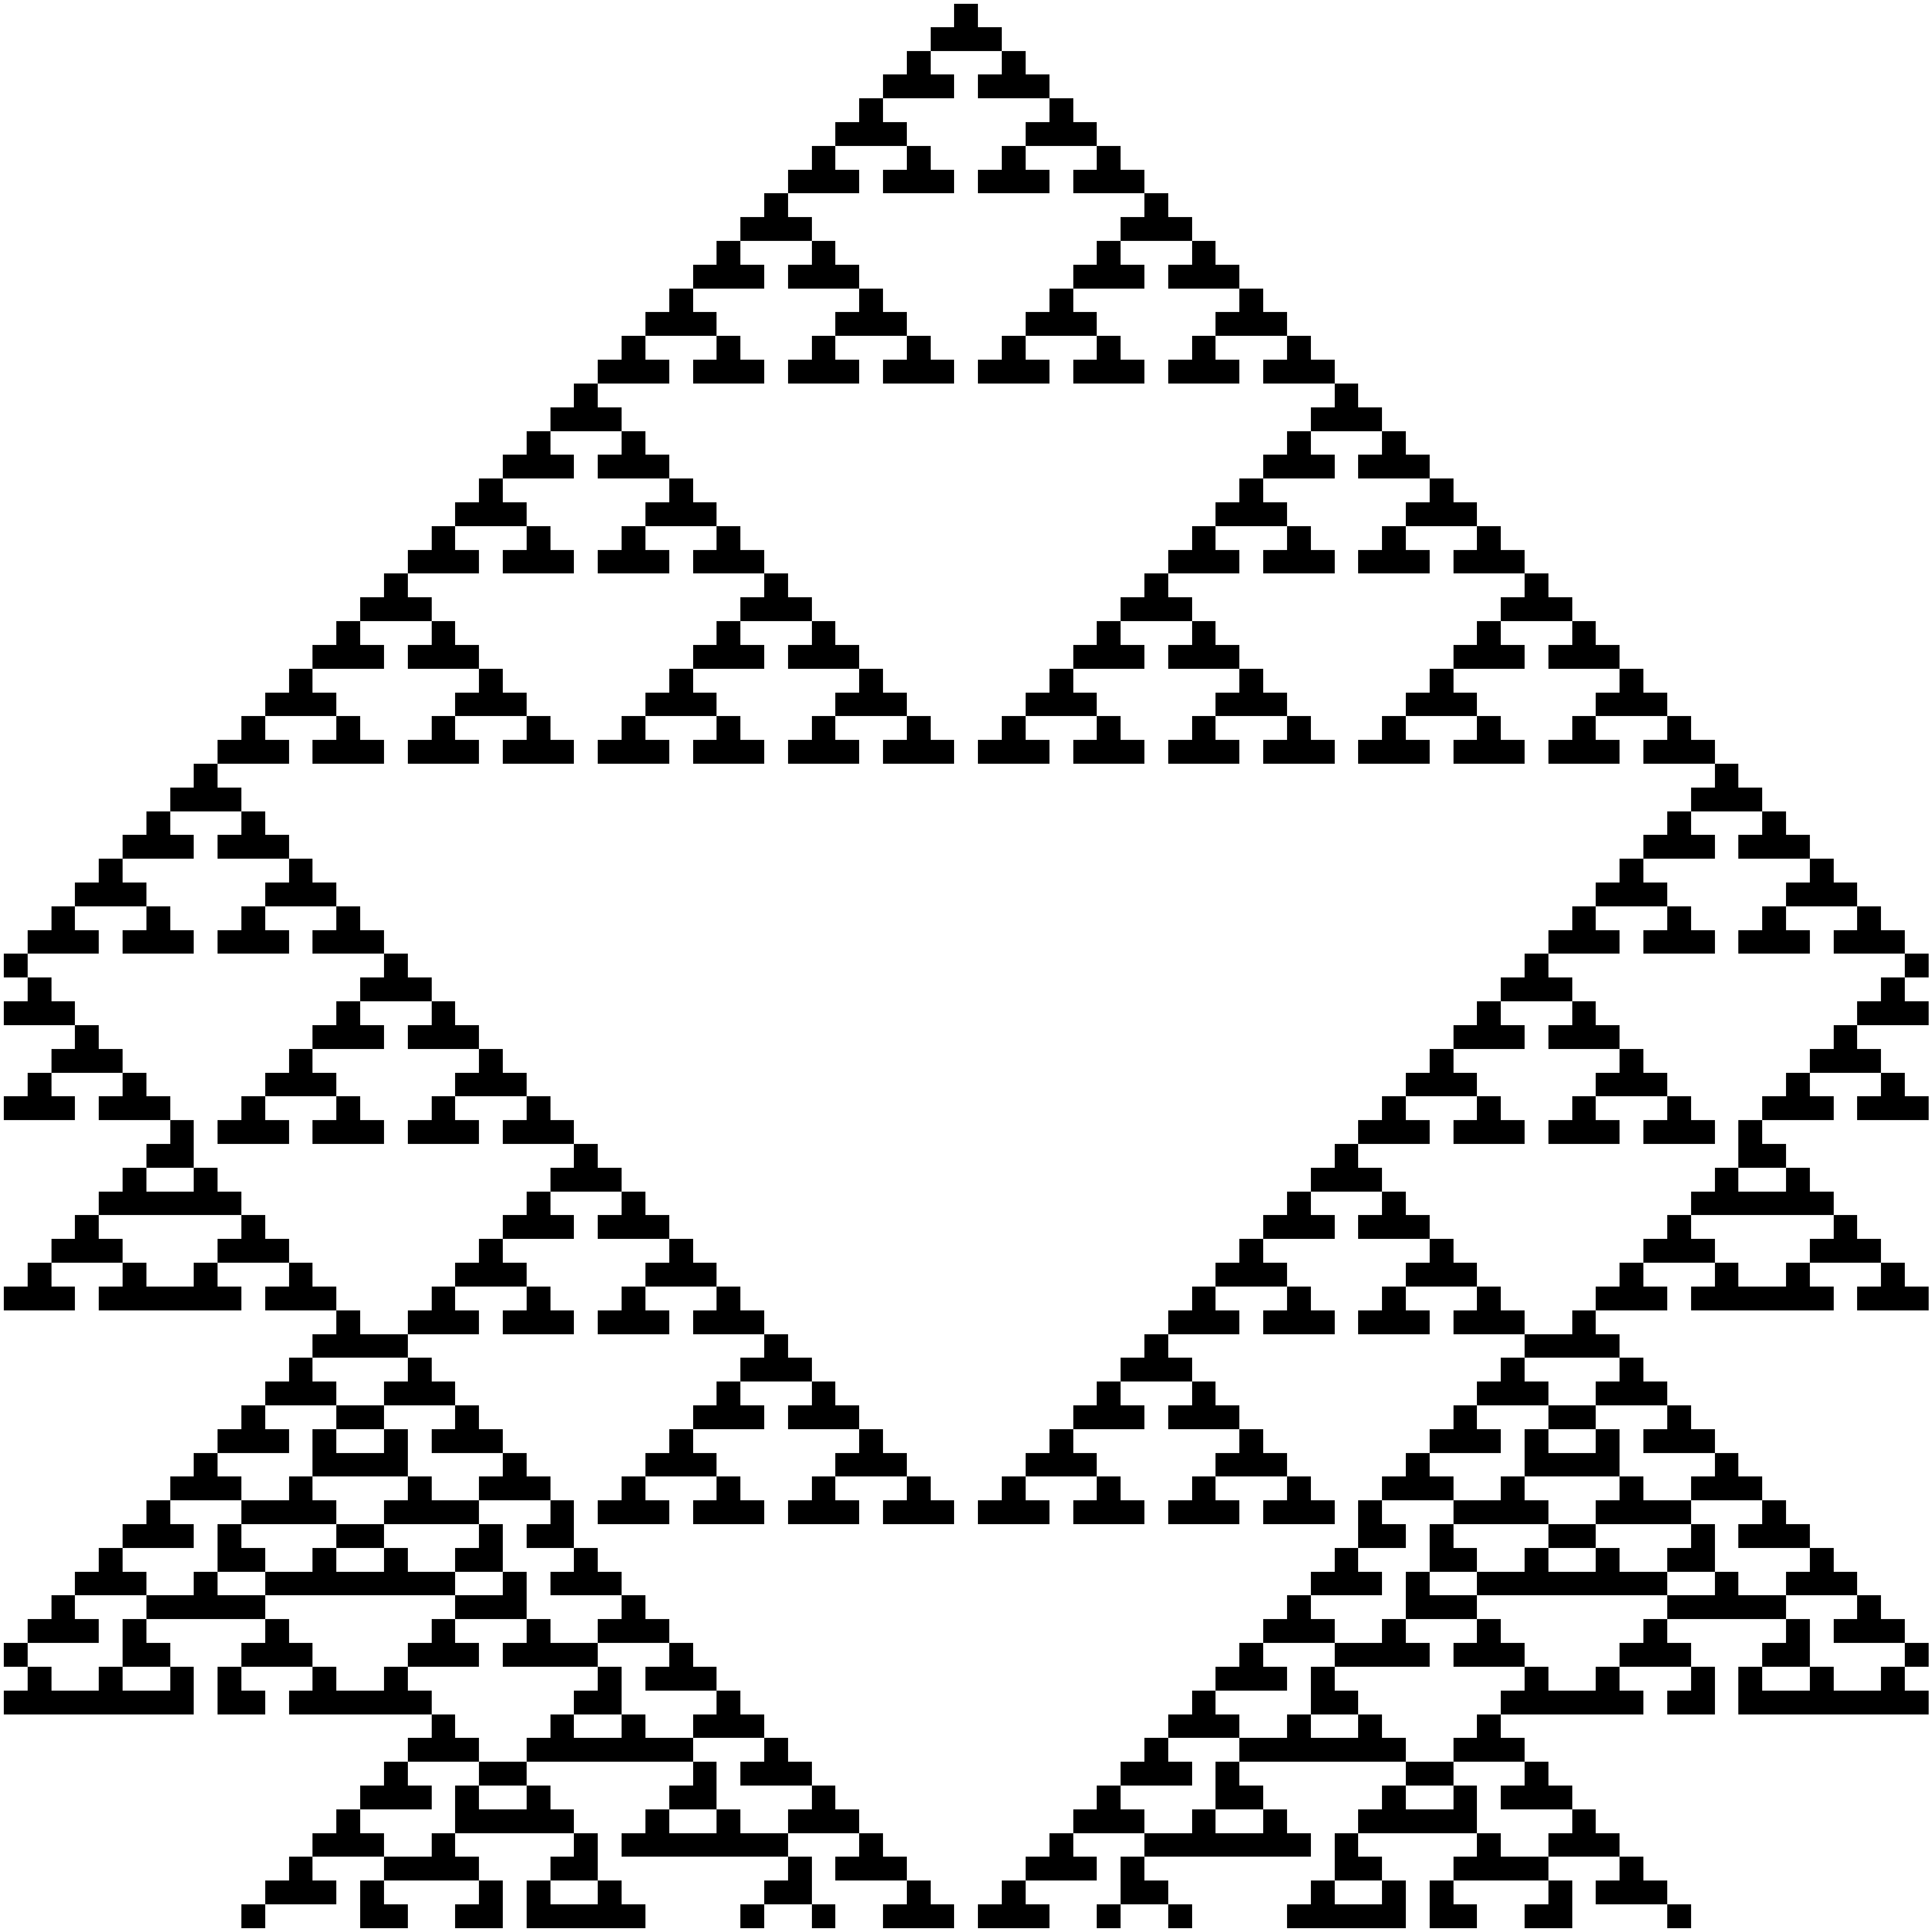
\includegraphics[width=8cm, height=8cm]{1d_plots/1d_rule_22.png}}
    \caption{Rule\_22; N=151, M=151}
    \label{fig:your_label}
\end{figure}

\vspace{0.5cm}

% Picture of rule 22
\begin{figure}[H]
    \centering
    \fbox{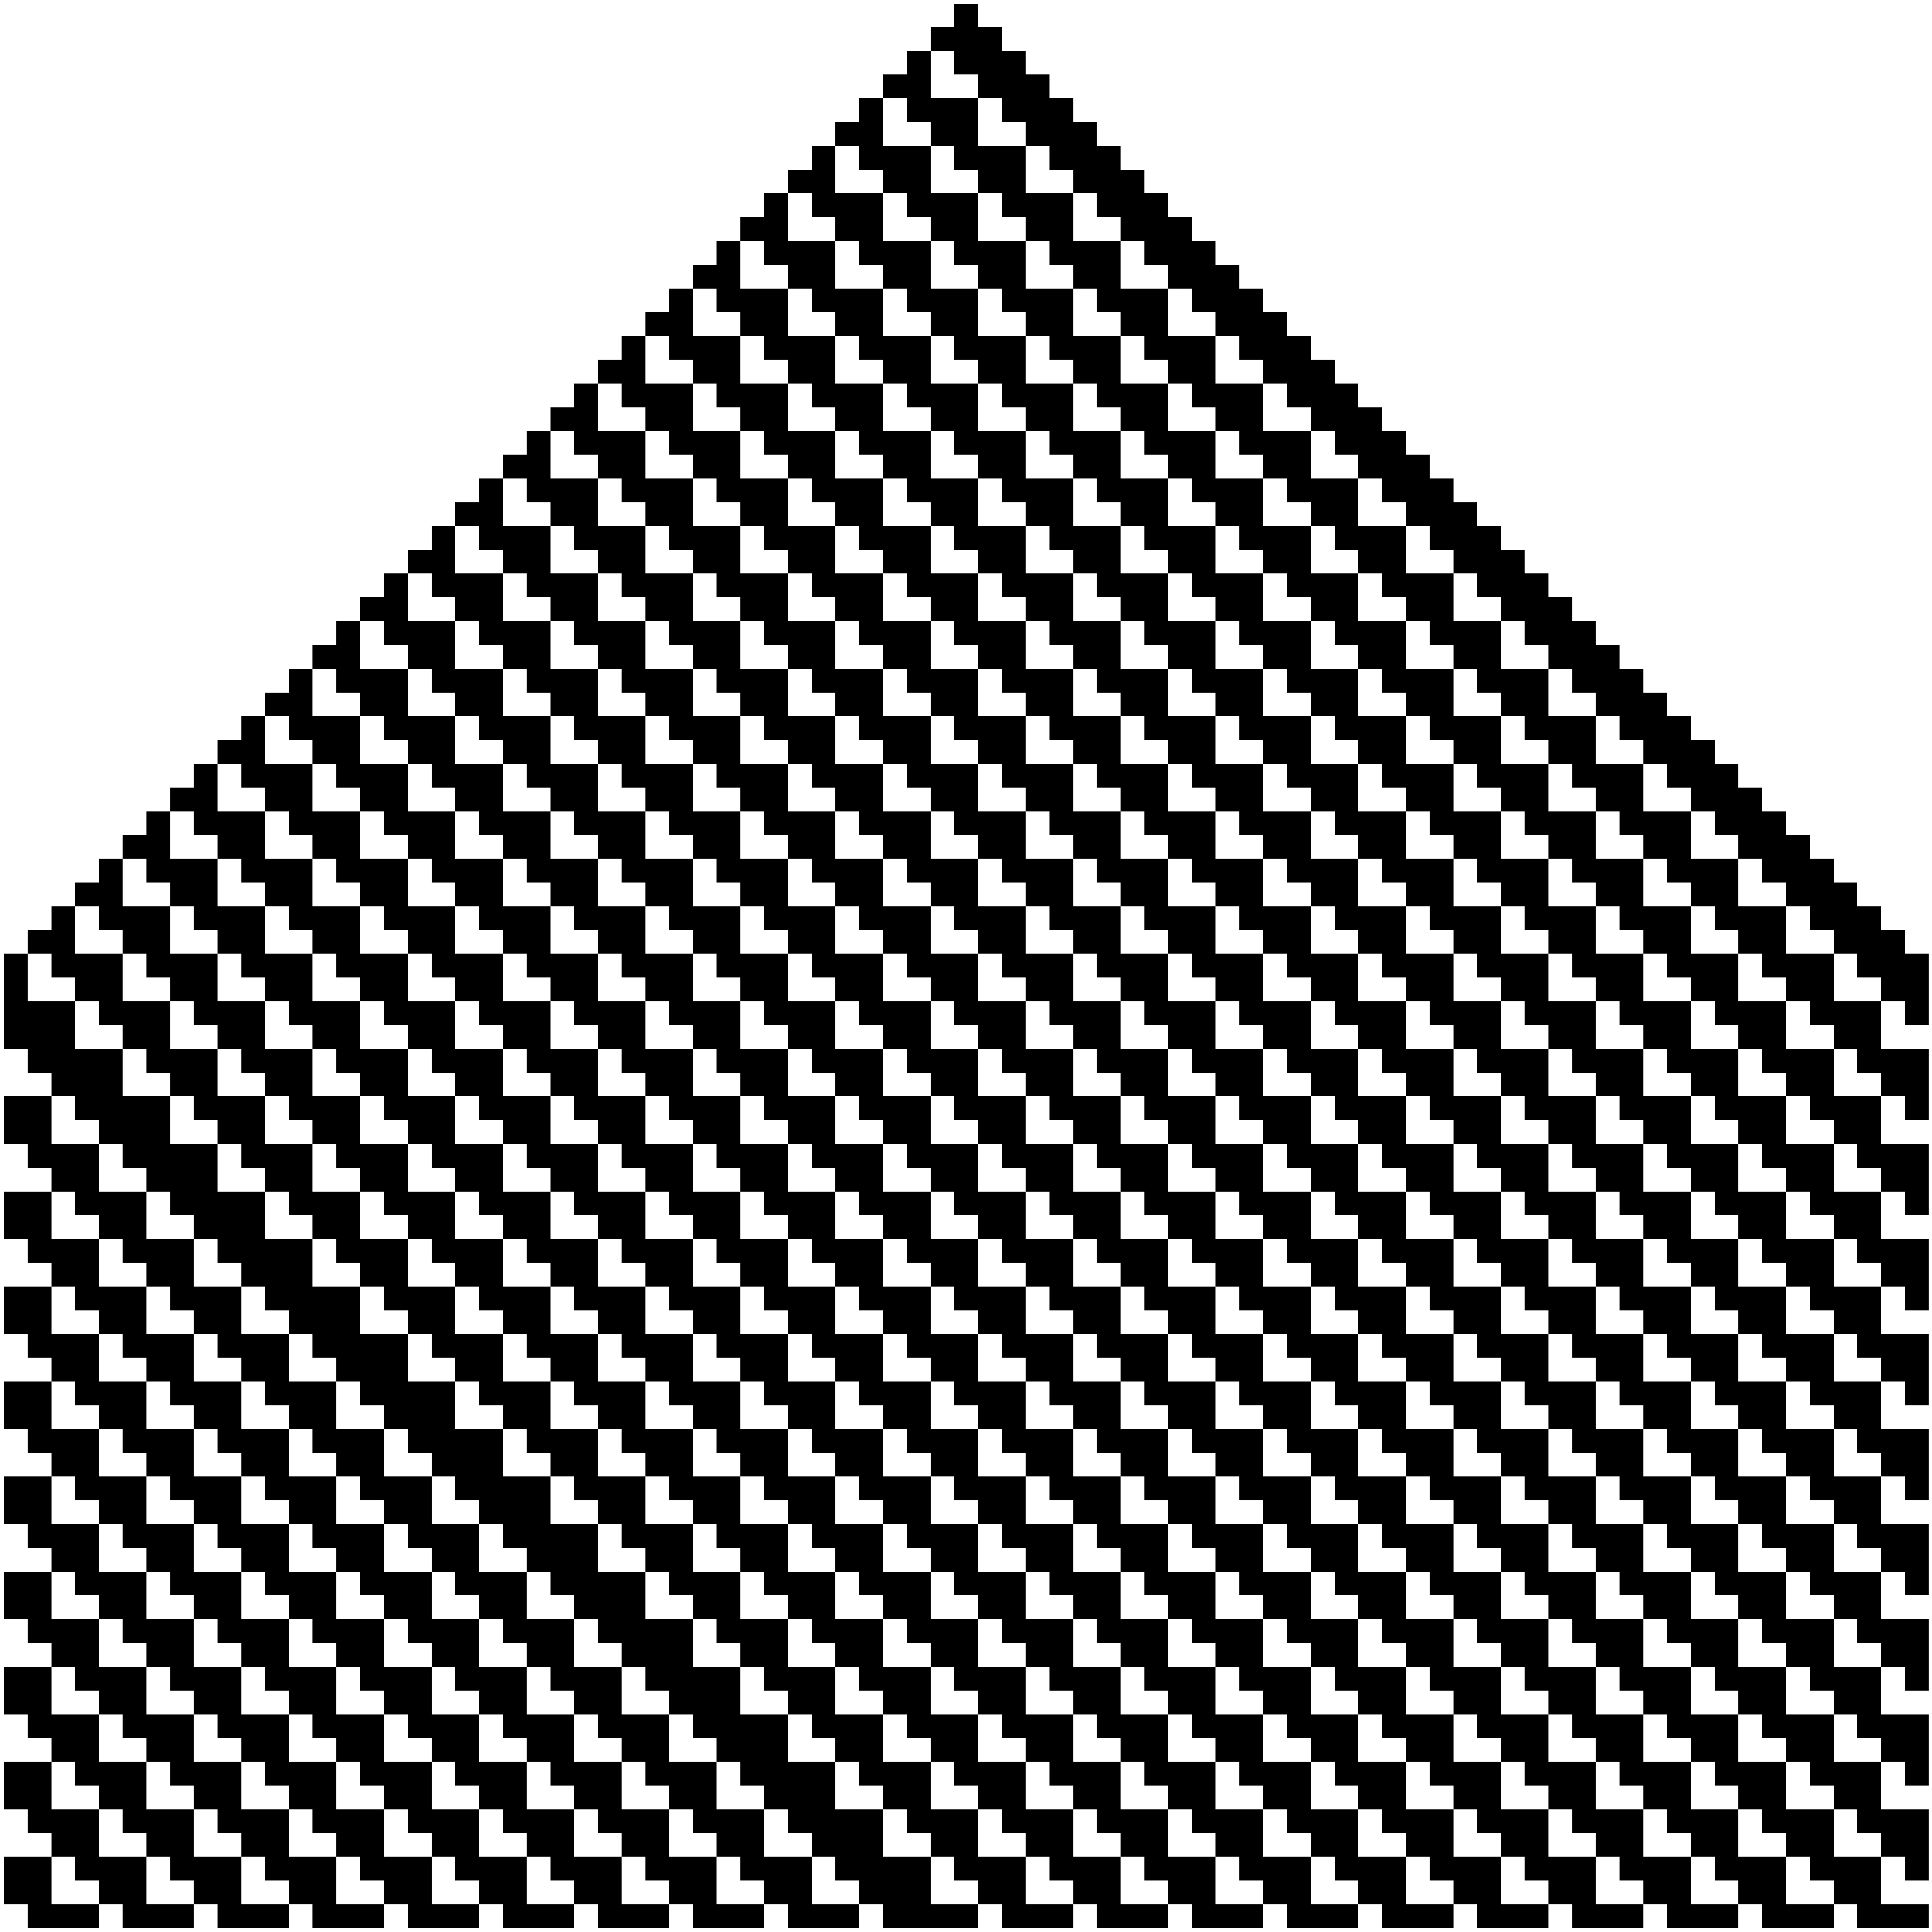
\includegraphics[width=8cm, height=8cm]{1d_plots/1d_rule_214.png}}
    \caption{Rule\_214; N=151, M=151}
    \label{fig:your_label}
\end{figure}

\newpage





% Problem B
\section{Part B}


\vspace{1cm}

\subsection{Idea}


\vspace{1cm}

\subsection{Implementation}


\vspace{1cm}

\subsection{Output}


\vspace{1cm}



\newpage


% Part D
\section{Pard D: Makefile}
\vspace{1cm}


\subsection{Function/struct distribution}
The goal of this part was to create several header files containing functions and structures used by the main programs.
\newline
We decided to create three header files:
\begin{enumerate}[label=\roman*.]
    \item \texttt{cell.h} - Contains functions for initializing and manipulating cellular automata.
    \item \texttt{stepcom.h} - Contains functions for computing and printing steps to files.
    \item \texttt{structs.h} - Contains struct definitions and rule declarations.
\end{enumerate}
The corresponding functions, rules, etc., are implemented in C files with the same names as the header files. 
For example, \texttt{cell.c} contains the functions declared in \texttt{cell.h}. Each header file is included in the main files 
to enable the use of the respective functions and structures.

\vspace{1cm}

\subsection{Makefile}
While the outsourcing of functions, structs, etc., improves code readability, it can complicate the compilation process. 
Fortunately, Makefiles simplify this task significantly by automating the build process.
\newline
\subsection*{\small Description}
This Makefile handles the entire build process for our cellular automata project. The all target is the main entry 
point, which compiles all three executables \texttt{(1dstates, 2d\_automat, and segler)}. To do that, we use a bunch of side rules 
— one for each object file — so every source file like \texttt{1d\_states.c, cell.c, structs.c}, and so on gets compiled separately 
into its own .o file first. The \texttt{CC} and \texttt{CFlags} variables up top help keep the compiler command \texttt{(gcc)} and options 
\texttt{(-Wall -Wextra -Wpedantic -std=c18)} consistent across all these targets.
\vspace{0.1cm}
We also added a run target to quickly compile and execute the main programs after a successful build. To use this command however, 
the user has to run the command \texttt{make run ARGS1="<n> <m>" ARGS2="<n> <m>"} where \texttt{<n>} is the size of the grid and 
\texttt{<m>} is the number of iterations. But be aware that \texttt{segler} has to be run seperately with \texttt{./segler} as it does not take any arguments.
Finally, there’s a clean target that deletes all the object files and executables so we can easily rebuild the project from scratch if needed.

\vspace{0.5cm}

% Makefile
\begin{lstlisting}[caption={\small Makefile},label={lst:p7001},basicstyle=\ttfamily\tiny,language=C]
    CC = gcc
    CFlags = -Wall -Wextra -Wpedantic -Wpedantic -std=c18

    # Main rule
    all: 1dstates 2d_automat segler

    # 1D cellular automats program
    1dstates: 1d_states.o cell.o structs.o stepcom.o
        $(CC) $^ -o $@

    1d_states.o: 1d_states.c cell.h structs.h stepcom.h
        $(CC) -c $(CFlags) $<

    cell.o: cell.c cell.h structs.h
        $(CC) -c $(CFlags) $<

    structs.o: structs.c structs.h
        $(CC) -c $(CFlags) $<

    stepcom.o: stepcom.c stepcom.h structs.h cell.h
        $(CC) -c $(CFlags) $<

    # Game of life program
    2d_automat: 2d_automat.o cell.o structs.o stepcom.o
        $(CC) $^ -o $@

    2d_automat.o: 2d_automat.c cell.h structs.h stepcom.h
        $(CC) -c $(CFlags) $<

    # Segler program
    segler: segler.o cell.o structs.o stepcom.o
        $(CC) $^ -o $@

    segler.o: segler.c cell.h stepcom.h
        $(CC) -c $(CFlags) $<


    run: 1dstates 2d_automat
        @./1dstates $(ARGS1)
        @./2d_automat $(ARGS2)


    .PHONY: all clean run
    clean:
        $(RM) *.o 1dstates 2d_automat segler
\end{lstlisting}


\newpage


% Code for all parts
\section{Appendix: Code and some more examples}

\subsection{Main files}

\subsection*{\small Part A - 1d\_states.c}
% Code 1d_states.c
\begin{lstlisting}[caption={\small 1d\_states.c},label={lst:p7001},basicstyle=\ttfamily\tiny]
    #include <stdio.h>
    #include <stdlib.h>
    #include <string.h>
    #include <time.h>

    // Own headers with function declarations, structs etc. 
    #include "structs.h"
    #include "cell.h"
    #include "stepcom.h"


    int main (int argc, char *argv[]) {
        if (argc != 3) {
            fprintf(stderr, "Usage: %s <n> <m>\n", argv[0]);
            return 1;
        }

        // User input for size and iterations
        int size = atoi(argv[1]);
        if (size <= 0) {
            fprintf(stderr, "Error: Size must be a positive integer.\n");
            return EXIT_FAILURE;
        }
        int iterations = atoi(argv[2]);

        // Initialize state
        cellauto *cell = malloc(sizeof(cellauto));
        if (!cell) {
            fprintf(stderr, "Error: Memory allocation failed.\n");
            return EXIT_FAILURE;
        }
        cell->state = malloc(size * sizeof(char));
        if (!cell->state) {
            fprintf(stderr, "Error: Memory allocation for state failed.\n");
            free(cell);
            return EXIT_FAILURE;
        }
        cell->rule = NULL; 
        cell->rule_name = 0;
        cell->rand = false;
        cell->iterations = iterations;
        cell->size = size;


        reset(cell); // Initialize state with a single '1' in the middle
        cell->rule = RULE_22;
        cell->rule_name = 22;

        // Compute steps for not random initial condition
        steps(cell);
        reset(cell); 
        cell->rule = RULE_106;
        cell->rule_name = 106;

        steps(cell);
        reset(cell); 
        cell->rule = RULE_187;
        cell->rule_name = 187;

        steps(cell);
        reset(cell); 
        cell->rule = RULE_214;
        cell->rule_name = 214;

        steps(cell);
        reset(cell); 


        // Now random states
        cell->rand = true;

        // Set random initial state
        srand(time(NULL)); // Seed for random number generation
        randomize(cell);
        cell->rule = RULE_22;
        cell->rule_name = 22;

        // Compute steps for random initial condition
        steps(cell);
        randomize(cell); 
        cell->rule = RULE_106;
        cell->rule_name = 106;

        steps(cell);
        randomize(cell); 
        cell->rule = RULE_187;
        cell->rule_name = 187;

        steps(cell);
        randomize(cell); 
        cell->rule = RULE_214;
        cell->rule_name = 214;

        steps(cell);

        // Free allocated memory
        free(cell->state);
        free(cell);

        return EXIT_SUCCESS;
    }
\end{lstlisting}


\vspace{1cm}

% Code 2d_automat.c
\subsection*{\small Part B - 2d\_automat.c}
\begin{lstlisting}[caption={\small 2d\_automat.c},label={lst:p7001},basicstyle=\ttfamily\tiny]
    #include <stdio.h>
    #include <stdlib.h>
    #include <time.h>

    // Self created headers
    #include "cell.h"
    #include "stepcom.h"


    int main(int argc, char *argv[])
    {
        if (argc != 3)
        {
            printf("Falsche Parameteranzahl, zwei werden benoetigt!\n");
            printf("Gittergroesse und Anzahl der Zeitschritte\n");
            exit(1);
        }

        int N = atof(argv[1]);
        int M = atof(argv[2]);

        srand(time(NULL));

        // Dynamically create array
        int **gitter = malloc(N * sizeof(int *));
        if (gitter == NULL)
        {
            fprintf(stderr, "Memory allocation failed for grid.\n");
            exit(1);
        }
        for (int i = 0; i < N; i++)
        {
            gitter[i] = malloc(N * sizeof(int));
            // Handle error correctly
            if (gitter[i] == NULL)
            {
                fprintf(stderr, "Memory allocation failed for grid row %d.\n", i);
                for (int j = 0; j < i; j++)
                {
                    free(gitter[j]);
                }
                free(gitter);
                exit(1);
            }
        }


        // Initialize the grid with random values
        random_auto((int **)gitter, N);


        // Compute time steps
        fileprint_auto((int **)gitter, N, M);


        // Free the allocated memory
        for (int i = 0; i < N; i++) {
            free(gitter[i]);
        }
        free(gitter);

        return 0;
    }
\end{lstlisting}


\vspace{1cm}

% Code segler.c
\subsection*{\small Part B - segler.c}
\begin{lstlisting}[caption={\small segler.c},label={lst:p7001},basicstyle=\ttfamily\tiny]
    #include <stdio.h>
    #include <stdlib.h>
    #include <time.h>

    #include "stepcom.h"
    #include "cell.h"


    int main()
    {
        int N = 200;
        int M = 200;

        // Dynamically create array
        int **gitter = malloc(N * sizeof(int *));
        if (gitter == NULL)
        {
            fprintf(stderr, "Memory allocation failed for grid.\n");
            exit(1);
        }
        for (int i = 0; i < N; i++)
        {
            gitter[i] = malloc(N * sizeof(int));
            // Handle error correctly
            if (gitter[i] == NULL)
            {
                fprintf(stderr, "Memory allocation failed for grid row %d.\n", i);
                for (int j = 0; j < i; j++)
                {
                    free(gitter[j]);
                }
                free(gitter);
                exit(1);
            }
        }

        // Initialize gitter with 0's
        for (int i = 0; i < N; i++)
        {
            for (int j = 0; j < N; j++)
            {
                gitter[i][j] = 0;
            }
        }

        // Spaceship
        int raumschiff[4][5] = {
            {0, 1, 0, 0, 1},
            {1, 0, 0, 0, 0},
            {1, 0, 0, 0, 1},
            {1, 1, 1, 1, 0}};

        // Place the spaceship in the grid
        for (int i = 0; i < 4; i++)
        {
            for (int j = 0; j < 5; j++)
            {
                gitter[i + 98][j + 150] = raumschiff[i][j];
            }
        }

        // Compute time steps
        fileprint_auto(gitter, N, M);

        // Free the allocated memory
        for (int i = 0; i < N; i++) {
            free(gitter[i]);
        }
        free(gitter);

        return 0;
}
\end{lstlisting}


\vspace{1cm}


\subsection{Headers}

% Code cell.h
\subsection*{\small cell.h}
\begin{lstlisting}[caption={\small cell.h},label={lst:p7001},basicstyle=\ttfamily\tiny,language=C]
    // Header for initializing and manipulating a cellular automats
    #ifndef CELL_H
    #define CELL_H

    #include "structs.h"

    void apply_rule (cellauto *cell);

    void reset (cellauto *cell);

    void randomize (cellauto *cell);

    int nachbar_check(int N, int row, int col, int **gitter);

    void random_auto( int **gitter, int size);

    #endif
\end{lstlisting}


\vspace{1cm}

% Code stepcom.h
\subsection*{\small stepcom.h}
\begin{lstlisting}[caption={\small stepcom.h},label={lst:p7001},basicstyle=\ttfamily\tiny,language=C]
    // Header for computing and printing steps into files
    #ifndef STEPCOM_H
    #define STEPCOM_H

    #include "structs.h"

    void steps(cellauto *cell);

    void fileprint_auto(int** gitter, int size, int steps);

    #endif
\end{lstlisting}


\vspace{1cm}

% Code structs.h
\subsection*{\small structs.h}
\begin{lstlisting}[caption={\small structs.h},label={lst:p7001},basicstyle=\ttfamily\tiny,language=C]
    // Header file for cellular automata structures
    #ifndef STRUCTS_H
    #define STRUCTS_H
    #include <stdbool.h>

    // Rules
    extern const char RULE_22[8];
    extern const char RULE_106[8];
    extern const char RULE_187[8];
    extern const char RULE_214[8];

    // Struct for states and rules
    typedef struct {
        char *state;
        // Rules are represented as strings of 8 characters
        const char *rule;  
        int rule_name;
        bool rand; // Random initial condition
        // Provided by input
        int iterations;  // Number of iterations
        int size;  // Size of the state
    } cellauto;

    #endif
\end{lstlisting}


\vspace{1cm}

\subsection{Header c-files}

% Code cell.c
\subsection*{\small cell.c}
\begin{lstlisting}[caption={\small cell.c},label={lst:p7001},basicstyle=\ttfamily\tiny,language=C]
    #include <stdio.h>
    #include <stdlib.h>

    #include "structs.h"
    #include "cell.h"

    // Fucntions for 1d automats


    // Function to apply the rule to the current state
    void apply_rule (cellauto *cell) {
        char new_state[cell->size];

        // Initialize new state with the current state
        for (int i = 0; i < cell->size; i++) {
            // Get the left, center, and right neighbors
            int left = cell->state[(i - 1 + cell->size) % cell->size] - '0';
            int center = cell->state[i] - '0';
            int right = cell->state[(i + 1) % cell->size] - '0';
            
            // Compute new state
            if (left == 1 && center == 1 && right == 1) {
                new_state[i] = cell->rule[0];
            }
            else if (left == 1 && center == 1 && right == 0) {
                new_state[i] = cell->rule[1];
            }
            else if (left == 1 && center == 0 && right == 1) {
                new_state[i] = cell->rule[2];
            }
            else if (left == 1 && center == 0 && right == 0) {
                new_state[i] = cell->rule[3];
            }
            else if (left == 0 && center == 1 && right == 1) {
                new_state[i] = cell->rule[4];
            }
            else if (left == 0 && center == 1 && right == 0) {
                new_state[i] = cell->rule[5];
            }
            else if (left == 0 && center == 0 && right == 1) {
                new_state[i] = cell->rule[6];
            }
            else { // left == 0 && center == 0 && right == 0
                new_state[i] = cell->rule[7];
            }
        }

        // Copy new state back to original state
        for (int i = 0; i < cell->size; i++) {
            cell->state[i] = new_state[i];
        }
    }

    // Function to reset the state to a single '1' in the middle
    void reset (cellauto *cell) {
        for (int i = 0; i < cell->size; i++) {
            cell->state[i] = '0';
        }

        int mid = cell->size / 2;
        cell->state[mid] = '1';
    }


    // Function to randomize the state
    void randomize (cellauto *cell) {
        for (int i = 0; i < cell->size; i++) {
            cell->state[i] = (rand() % 2) + '0'; // Randomly set '0' or '1'
        }
    }


    // Functions for 2d automats


    // Function to check the number of neighbors for a cell at (row, col) in a grid of size N
    int nachbar_check(int N, int row, int col, int **gitter) {
        int one_counter = 0;

        for (int i = row - 1; i < row + 2; i += 2)
        {
            for (int j = col - 1; j < col + 2; j++)
            {
                if (i > -1 && i < N && j > -1 && j < N)
                {
                    if (gitter[i][j] == 1)
                    {
                        one_counter++;
                    }
                }
            }
        }

        for (int j = col - 1; j < col + 2; j += 2)
        {
            if (j > -1 && j < N)
            {
                if (gitter[row][j] == 1)
                {
                    one_counter++;
                }
            }
        }

        return one_counter;
    }


    // Function to fill the grid with random values (0 or 1)
    void random_auto( int **gitter, int size) {
        for (int i = 0; i < size; i++)
        {
            for (int j = 0; j < size; j++)
            {
                gitter[i][j] = rand() % 2;
            }
        }
    }
\end{lstlisting}


\vspace{1cm}

% Code stepcom.c
\subsection*{\small stepcom.c}
\begin{lstlisting}[caption={\small stepcom.c},label={lst:p7001},basicstyle=\ttfamily\tiny,language=C]
    #include <stdio.h>
    #include <stdlib.h>
    #include <sys/stat.h>   // for mkdir

    #include "stepcom.h"
    #include "cell.h"

    // Fucntions for 1d automats


    // Function for computing iterated steps
    void steps(cellauto *cell) {
        // 1. Check if the folder exists, do not create a new one
        struct stat st;
        if (stat("1d_plots", &st) != 0 || !S_ISDIR(st.st_mode)) {
            fprintf(stderr, "Error: Folder '1d_plots' does not exist.\n");
            exit(1);
        }

        // 2. Build the filename: e.g., "1d_plots/1d_rule_187.txt" for different states
        char filename[256];
        if (!cell->rand) {
            snprintf(filename, sizeof(filename),
                "1d_states/1d_rule_%d.txt",
                cell->rule_name);
        }
        else {
            snprintf(filename, sizeof(filename),
                "1d_states/1d_rule_%d_random.txt",
                cell->rule_name);
        }

        // 3. Open the file for writing
        FILE *file = fopen(filename, "w");
        if (!file) {
            perror("fopen");
            exit(1);
        }

        // 4. Example: write the initial state
        for (int i = 0; i < cell->size; i++) {
            fputc(cell->state[i], file);
            if (i + 1 < cell->size) fputc(' ', file);   
        }
        fputs("\n", file);

        // 5. Iteration loop to apply the rule and write the states
        for (int it = 1; it < cell->iterations; it++) {
            // Apply rule
            apply_rule(cell);
            // Write the new state to the file
            for (int i = 0; i < cell->size; i++) {
                fputc(cell->state[i], file);
                if (i + 1 < cell->size) fputc(' ', file);
            }
            fputs("\n", file);
        }

        fclose(file);
    }


    // Functions for 2d automats


    // Funtion for prinitng the states into files
    void fileprint_auto(int** gitter, int size, int steps) {
        for (int t = 0; t < steps; t++)
        {
            int temp[size][size];
            for (int i = 0; i < size; i++)
            {
                for (int j = 0; j < size; j++)
                {
                    if (gitter[i][j] == 1)
                    {
                        if (nachbar_check(size, i, j, gitter) < 2)
                        {
                            temp[i][j] = 0;
                        }
                        else if (nachbar_check(size, i, j, gitter) > 3)
                        {
                            temp[i][j] = 0;
                        }
                        else
                        {
                            temp[i][j] = 1;
                        }
                    }
                    else
                    {
                        if (nachbar_check(size, i, j, gitter) == 3)
                        {
                            temp[i][j] = 1;
                        }
                        else
                        {
                            temp[i][j] = 0;
                        }
                    }
                }
            }
            for (int i = 0; i < size; i++)
            {
                for (int j = 0; j < size; j++)
                {
                    gitter[i][j] = temp[i][j];
                }
            }

            FILE *file;

            char filename[50];
            snprintf(filename, sizeof(filename), "2d_states/2d_state_%04d.txt", t + 1);

            file = fopen(filename, "w");

            for (int i = 0; i < size; i++)
            {
                for (int j = 0; j < size; j++)
                {
                    fprintf(file, "%d ", gitter[i][j]);
                }
                fprintf(file, "\n");
            }
            fclose(file);
        }
    }
\end{lstlisting}


\vspace{1cm}

% Code structs.c
\subsection*{\small structs.c}
\begin{lstlisting}[caption={\small structs.c},label={lst:p7001},basicstyle=\ttfamily\tiny,language=C]
    // Define rules
    const char RULE_22[8] = {'0', '0', '0', '1', '0', '1', '1', '0'}; // 22 in binary
    const char RULE_106[8] = {'0', '1', '1', '0', '1', '0', '1', '0'}; // 106 in binary
    const char RULE_187[8] = {'1', '0', '1', '1', '1', '0', '1', '1'}; // 187 in binary
    const char RULE_214[8] = {'1', '1', '0', '1', '0', '1', '1', '0'}; // 214 in binary
\end{lstlisting}

\end{document}